\documentclass[12pt,a4paper]{article}
\usepackage{graphicx} % Required for inserting images
\usepackage{authblk}
\usepackage{hyperref}
\usepackage{sectsty}
\usepackage{enumerate}
\usepackage{graphicx}
\usepackage{float}
\usepackage{xspace}
\usepackage[long]{datetime}
\usepackage{listings}
\usepackage{xcolor}
\usepackage{amsmath}
\usepackage[style=numeric,sorting=none]{biblatex}
\addbibresource{references.bib}

\numberwithin{figure}{subsection}

\lstdefinestyle{shortcode}{
  basicstyle=\ttfamily\small,
  breaklines=true,
  columns=fullflexible,
  showstringspaces=false,
}

\hypersetup{
	colorlinks=true,
	allcolors=blue,
}
\setlength{\textheight}{241 mm}  \setlength{\textwidth}{159.2 mm}
\setlength{\oddsidemargin}{0 pt} \setlength{\evensidemargin}{0 pt}
\setlength{\topmargin}{-20 mm}   \setlength{\headheight}{10 mm}
\setlength{\headsep}{10 mm}      %\setlength{\parindent}{0 pt}
\setlength{\parskip}{1ex plus 0.5ex minus 0.2ex}

\allsectionsfont{\sffamily} %from sectsty package

\graphicspath{ {./figures/} }

\newcommand{\todo}[1]{{\textcolor{red}{\sf{[TODO: #1]}} }}
\newcommand{\mr}[1]{{\textcolor{cyan}{\sf{[MR: #1]}} }} %Mr who?
\newcommand{\kc}[1]{{\textcolor{magenta}{\sf{[KC: #1]}} }}
\newcommand{\el}[1]{{\textcolor{blue}{\sf{[EL: #1]}} }}

% Codes
\newcommand{\bam}{\textsc{BAM}\xspace}
\newcommand{\einsteintoolkit}{\textsc{Einstein Toolkit}\xspace}
\newcommand{\etk}{\textsc{ETK}\xspace} % This doesn't do anything but here for completeness
\newcommand{\exagrype}{\textsc{ExaGRyPE}\xspace}
\newcommand{\grteclyn}{\textsc{GRTeclyn}\xspace}
\newcommand{\mhduet}{\textsc{MHDuet}\xspace}

% Code libraries/dependencies
\newcommand{\amrex}{\textsc{AMReX}\xspace}
\newcommand{\carpet}{\textsc{Carpet}\xspace}
\newcommand{\carpetx}{\textsc{CarpetX}\xspace}
\newcommand{\exahype}{\textsc{ExaHyPE}\xspace}
\newcommand{\peano}{\textsc{Peano}\xspace}
\newcommand{\simflowny}{\textsc{Simflowny}\xspace}


\title{UKNR CCP: Numerical Relativity Code Assessment}

\author[1]{Miren Radia}
\affil[1]{University of Cambridge}
\author[2]{Eugene Lim}
\affil[2]{King's College London}
\author[3]{Katy Clough}
\affil[3]{Queen Mary University of London}
\author[4]{Mark Hannam}
\affil[4]{Cardiff University}

\date{\today}

\setcounter{Maxaffil}{0}
\renewcommand\Affilfont{\itshape\small}

\begin{document}

\maketitle

%=============================================================================
\section{Introduction}

Several different 3+1 numerical relativity (NR) codes are being used and developed
by members of the UKNR community. These codes employ a variety of
infrastructure, numerical methods and parallelisation strategies, and they
differ in their capabilities, maturity and performance. While
there have been some efforts to compare codes, most of these
have focused on just two codes and the physical results they produce rather
than their usability, development status and performance.

The UKNR community has been provided with funding to develop its status towards becoming a
Collaborative Computational Project (CCP). As part of this we felt it was important to understand the
current state of the codes that are being used. Key questions include:
\begin{itemize}
    \item What are their methods and capabilities (beyond physics)?
    \item What are they like to use and get started with?
    \item For codes that are currently under active development, what is their
    current development status?
    \item How do they perform?
\end{itemize}
This report documents a code assessment exercise that was carried out to
address these questions.

\subsection{Limitations of this assessment}

Given finite time, there were many things we were not able to investigate. A
non-exhaustive list of these includes:
\begin{itemize}
    \item Matter: when assessing performance, we considered vacuum black hole spacetimes only, since not all
    of the codes support the same types of matter.
    \item We did not test every feature and capability of each code.
    \item We did not validate the accuracy of the results produced by the codes.
    \item Rigorous performance comparisons between codes: our performance tests
    were not designed to compare codes directly against each other on
    like-for-like problems, but rather intended to give a rough idea of how codes performed on
    a similar problem type (the binary black hole) and identify any major differences.
    \item Weak scaling: we only performed strong scaling tests.
\end{itemize}
Furthermore, this assessment is a snapshot in time: many of the codes are
under active development, so their capabilities, usability and performance are
subject to change.

\subsection{Contents of this report}

This report is organised as follows. In Sec.~\ref{sec:codes}, we describe the
codes we assessed and their current capabilities, including their numerical and
mathematical methods. In Sec.~\ref{sec:hpc}, we briefly describe the DiRAC HPC
systems (COSMA8 and Tursa) that were used for testing. In
Sec.~\ref{sec:usability}, we document our qualitative experiences of obtaining,
building and using each code. In Sec.~\ref{sec:performance}, we present the
results of strong scaling tests and profiling of the codes. Finally, we
summarise our findings in Sec.~\ref{sec:conclusion}.

%=============================================================================
\section{The codes and their current capabilities}
\label{sec:codes}

In this section, we describe the current state of the NR codes that we assessed
as part of this exercise. Although there are many other codes that are used
internationally,  we have chosen to only consider those that met the following
criteria:
\begin{enumerate}
    \item The code has some relevance within the UKNR community. For example,
    there is at least one developer based in the UK or there are several active UK users.
    \item The code is capable of evolving in 3+1 dimensions (i.e. it is not
    dimensionally reduced and does not require the use of symmetries).
    \item The code is capable of evolving a binary-black hole spacetime through
    inspiral, merger and ringdown.
\end{enumerate}
Based on these criteria, we assess the following codes:
\begin{itemize}
    \item \bam
    \cite{Bruegmann:1997uc,Bruegmann:2003aw,Husa:2007hp,Bruegmann:2006ulg}
    \item The \einsteintoolkit(\etk) \cite{Loffler:2011ay,EinsteinToolkit:2025_05}
    \item \exagrype \cite{Zhang:2024fye}
    \item \grteclyn \cite{GRTeclyn:2026}
    \item \mhduet \cite{Palenzuela:2025ucx}
\end{itemize}
Note that this list is not exhaustive. For example, we have not
included \textsc{GRChombo} \cite{Clough:2015sqa,Andrade:2021rbd} because it is
anticipated that \grteclyn will replace it in the next few years.

All of these codes use the following common methods:
\begin{itemize}
    \item Finite differences
    \item Mesh refinement where the computational domain consists of a hierarchy
    of levels with each level comprising Cartesian grids with a fixed grid
    spacing which becomes progressively smaller as you go up the hierarchy.
    Each level covers a subset of the domain of the coarser level immediately
    below it with the coarsest level covering the whole computational domain.
    \item Method of Lines with fourth-order Runge Kutta (RK4) time integration
    \item 3+1 evolution system: either BSSN, CCZ4 or Z4c typically with some
    variation of the Moving Puncture gauge conditions
    \cite{Campanelli:2005dd,Baker:2005vv}.
    \item Kreiss-Oliger dissipation \cite{Kreiss:1973}.
\end{itemize}
Furthermore, they are all parallelised using the Message Passing Interface
(MPI).

\subsection{BAM}

\subsubsection{Properties and structure}
\bam has the following properties:
\begin{itemize}
    \item It is written in C.
    \item It is purely MPI parallelized with no additional hybrid
    parallelization.
    \item It uses \textsc{Make} to build with a separate config file to
    configure the build for the local system and required features.
    \item It has very few dependencies: a C compiler, \textsc{Make}, and an MPI
    implementation with optional HDF5 support.
    \item It was originally written in the mid-90s by Bernd Br\"ugmann, but the
    version we consider reached close to its current form in the mid-2000s and
    has not changed significantly since then.
    \item Inspired by the Einstein Toolkit, it has a modular design. The code is
    split up into libraries that are organised into folders, and different
    features can be enabled or disabled when configuring the build.
\end{itemize}

\subsubsection{Numerical methods}
\bam uses the following numerical methods:
\begin{itemize}
    \item It uses node/vertex-centred stencils.
    \item It employs moving-box-style mesh refinement, where the finest few
    levels consist of boxes centred on each black hole. During regridding, the
    boxes are moved such that their centres coincide with the tracked punctures.
    \item Berger-Oliger subcycling \cite{Berger:1984zza} is used for most of the
    levels but is typically disabled for some coarser levels in order to allow
    evolving very large domains with correspondingly large grid spacings without
    triggering an instability.
    \item It uses sixth order spatial differencing with eighth order
    Kreiss-Oliger dissipation.
\end{itemize}

\subsubsection{Mathematical methods}
\bam uses the following mathematical methods:
\begin{itemize}
    \item It uses the BSSN evolution scheme.
    \item It employs the moving puncture gauge conditions.
    \item It enforces algebraic constraints.
    \item It applies radiative/Sommerfeld boundary conditions.
\end{itemize}

\subsubsection{Additional capabilities}
\bam has the following additional capabilities:
\begin{itemize}
    \item It supports puncture tracking.
    \item It includes an apparent horizon (AH) finder.
    \item It supports grid symmetries (e.g. bitant, quadrant, octant, etc.).
    \item It can interpolate grid variables using fourth or sixth order Lagrange
    polynomials.
    \item It can compute $\Psi_4$ and extract gravitational waves via the
    Newman-Penrose formalism \cite{Newman:1961qr}.
\end{itemize}

\subsection{Einstein Toolkit}
\begin{itemize}
    \item The \einsteintoolkit is built on the Cactus Computational Toolkit
    (CCTK) \cite{Goodale2002a}, which is a software framework for solving PDEs.
    \item A CCTK code comprises the Cactus \emph{flesh} with some additional
    \emph{thorns} that implement a specific problem.
    \item The \einsteintoolkit is not really a single code in itself but rather
    just a collection of thorns with the Cactus flesh that can be used for NR
    problems. For example, several possible thorns are available that implement
    the the right-hand side calculation for the BSSN equations.
    \item Thorns can be written in C, C++ or Fortran but they have a
    standardized interface which describes their parameters, the C functions
    they export/provide to other thorns, any functions/thorns they depend on,
    when their functions are scheduled during a simulation, and any public
    variables.
    \item The recommended way to build, manage and run simulations with the
    Einstein Toolkit is with the \textsc{SimFactory2} thorn which provides an
    abstraction layer over different HPC systems. It requires that the machine
    you are using is configured in its database.
    \item One of the core thorns is the \emph{driver} which implements the
    computational grid, mesh refinement and associated
    infrastructure\footnote{This is assuming you use a driver which supports
    mesh refinement. The default Cactus driver is PUGH which is a unigrid
    driver.}.
    \item The most popular and well-supported driver is \carpet
    \cite{Schnetter:2003rb} which was developed in the early 2000s. This works just on CPUs.
    \item The next-generation replacement for \carpet is \carpetx
    \cite{Shankar:2022ful} which is built on the \amrex
    \cite{Zhang:2019a,Zhang:2021a} framework for block-structured AMR.
    \item \carpet supports OpenMP parallelisation whereas \carpetx supports
    OpenMP parallelization and offloading to Nvidia GPUs via CUDA. In principle,
    \amrex supports offloading to AMD and Intel GPUs though this is not
    currently explicitly exposed.
\end{itemize}
We used different thornlists for our CPU and GPU tests. For our CPU tests, we
used the following configuration:
\begin{itemize}
    \item A subset of the thorns from the \etk 2025\_05 Kruskal release
    \cite{EinsteinToolkit:2025_05} was selected.
    \item The \carpet mesh refinement driver was used.
    \item Evolution was performed using the \textsc{McLachlan} BSSN evolution
    thorns \cite{Brown:2008sb,Husa:2004ip}.
    \item Eighth order spatial differencing was employed.
    \item Subcycling was performed using buffer zones, with fifth order
    prolongation (interpolation from coarse to fine) in space and second order
    prolongation in time.
    \item Moving-box-style mesh refinement was provided by the
    \textsc{CarpetRegrid2} thorn.
    \item Sommerfeld boundary conditions were provided by the \textsc{ML\_BSSN}
    thorn.
\end{itemize}
For our GPU tests, we used the following configuration:
\begin{itemize}
    \item Recent development versions of the \carpetx and \textsc{SpacetimeX}
    thorns by Liwei Ji were used, which support subcycling in time \cite{Ji:2025rpd}.
    This was intended to make the performance comparison more representative,
    since subcycling is used by most of the other codes, but we note that the
    implementation was not yet merged with the main CarpetX code at the time of testing.
    \item The \carpetx mesh refinement driver was used.
    \item Evolution was performed using the Z4c evolution thorn from
    \textsc{SpacetimeX}.
    \item Fourth order spatial differencing was employed.
    \item Subcycling was performed with fifth order prolongation.
    \item Moving-box-style mesh refinement was provided by the
    \textsc{BoxInBox} thorn.
    \item Sommerfeld boundary conditions were provided by the \textsc{NewRadX}
    thorn.
\end{itemize}
There are many additional capabilities (sometimes available with multiple
implementations in different thorns) available in the \einsteintoolkit. These
include:
\begin{itemize}
    \item Multipatch support with ``cubed sphere'' patches surrounding the main
    Cartesian domain is provided by the \textsc{Llama}
    \cite{Pollney:2009yz} infrastructure thorns for \carpet and by the
    \textsc{CapyrX} \cite{Sanches:2026a} infrastructure thorn for \carpetx. We
    did not use this capability in order to make a fairer comparison with other
    codes.
    \item Puncture tracking is provided by the \textsc{PunctureTracker} thorn.
    \item Apparent horizon finding is provided by the \textsc{AHFinder},
    \textsc{AHFinderDirect} \cite{Thornburg:1995cp} and \textsc{ET\_BHaHAHA}
    \cite{Etienne:2025auk} thorns.
    \item Computation of $\Psi_4$ is provided by the \textsc{WeylScal4} and
    \textsc{NPScalar} thorns, and its decomposition into modes relative to the
    spin-weighted spherical harmonics is provided by the \textsc{Multipole}
    thorn.
    \item Lagrange polynomial interpolation of grid variables is available
    using the \textsc{CarpetInterp} or \textsc{CarpetInterp2} thorns and the
    \textsc{AEILocalInterp} thorn in the \carpet case, or as a core \carpetx
    capability in that case.
    \item Reflection and rotation grid symmetries are supported.
    \item Output of data compatible with the SpECTRE Cauchy Characteristic
    Extraction code \cite{Moxon:2021gbv} is provided by the \textsc{CCE\_Export}
    thorn.
    \item Many thorns that were originally written for use with \carpet have
    been rewritten with support for \carpetx. As with the driver, these are
    usually renamed with an X suffix, for example \textsc{TwoPunctures}
    \cite{Ansorg:2004ds} and \textsc{TwoPuncturesX}.
\end{itemize}
This list is far from exhaustive.

\subsection{ExaGRyPE}

\subsubsection{Code structure}
\begin{itemize}
    \item \exagrype is an NR code built upon \textsc{ExaHyPE} 2 (second
    generation Exascale Hyperbolic Partial Differential Equation Engine)
    \cite{Reinarz:2020a} which in turn is built upon \textsc{Peano}
    \cite{Weinzierl:2019a}, an open-source framework for solvers on dynamically
    adaptive Cartesian meshes.
    \item \exagrype, \textsc{ExaHyPE} 2 and \textsc{Peano} are written in a mix
    of C++ and Python with more C++ at the bottom of the stack (i.e. at the
    \textsc{Peano} end) and more Python at the top of stack (i.e. at the
    \exagrype end).
    % \item To build an \exagrype simulation executable, a Python script is
    % invoked. Note that unlike in other codes, parameters are set using arguments
    % to the Python build script and cannot be changed at runtime. The executable
    % can then be launched using the standard MPI launcher (e.g.
    % \texttt{mpiexec}) without any arguments.
    \item Unlike other codes that are distributed using domain decomposition
    with any additional parallelization being data parallelism, \exagrype is
    parallelized using a mix of domain decomposition and task-based parallelism:
       \begin{itemize}
           \item As usual, distributed parallelism is handled using MPI.
           \item On CPUs, \textsc{Peano}/\textsc{ExaHyPE} 2 supports using its
           tasked-based parallelism  via C++ threading, Intel Threaded Building
           Blocks, OpenMP or SYCL.
           \item They support offloading to GPUs via SYCL and OpenMP which are
           both vendor-agnostic.
           \item Although both \textsc{Peano} and \textsc{ExaHyPE} 2 may support
           these programming models, support within \exagrype is not guaranteed
           and may not work.
       \end{itemize}
    \item The design of \exagrype is to aim for a separation of concerns. The
    scientific user should only need to use the Python domain-specific language
    (DSL) with the handling of the technical details including scheduling,
    task-distribution, looping over the domain, etc performed by the
    \textsc{ExaHyPE} engine.
\end{itemize}

\subsubsection{Numerical methods}
\exagrype uses the following numerical methods:
\begin{itemize}
    \item It uses cell-centred stencils.
    \item The computational domain consists of Cartesian blocks which are
    constructed using a spacetree formalism. The whole domain is embedded into a
    single cube and split into three equally along each coordinate axis to give
    $3^3 = 27$ smaller cubes\footnote{In the alternative case where each cube is
    split into two along each coordinate axis, this is commonly referred to as
    the \emph{Octtree} formalism. Using $3$ instead of $2$ is chosen here so
    that cell centres between coarser and refined cells co-incide.}. These cubes
    are then recursively refined with a problem-specific refinement criteria
    determining when to stop refining.
    \item It uses fourth-order spatial differencing.
    \item It uses explicit Runge-Kutta (RK) time integration. Up to fourth order
    RK is supported, but first order is used by default with a smaller timestep
    for computational efficiency.
    \item It employs sixth-order Kreiss-Oliger dissipation.
    \item It uses trilinear interpolation from coarse to fine cells.
    \item It uses cell averaging for restriction/interpolation from fine to
    coarse cells.
\end{itemize}

\subsubsection{Mathematical methods}
\exagrype uses the following mathematical methods:
\begin{itemize}
    \item It uses the CCZ4 evolution scheme that is recast as
    first-order-in-space, resulting in 58 evolution variables.
    \item CCZ4 algebraic constraints are enforced after each timestep.
    \item It uses the standard moving-puncture gauge conditions.
    \item It applies Sommerfeld boundary conditions (BCs) by default.
    \item It uses Bowen-York initial data provided by \textsc{TwoPunctures}
    \cite{Ansorg:2004ds}.
\end{itemize}

\subsubsection{Additional capabilities}
\exagrype has the following additional capabilities:
\begin{itemize}
    \item It supports trilinear interpolation from grid values onto particle
    tracers.
    \item It computes $\Psi_4$ and extracts gravitational waves via the
    Newman-Penrose formalism using the above particle tracer interpolation.
    \item It supports puncture tracking using particle tracer interpolation.
\end{itemize}

\subsection{GRTeclyn}

\subsubsection{Properties and structure}
\grteclyn has the following properties:
\begin{itemize}
    \item It is written in modern C++ (C++20 is required, but mostly C++14/17
    features are used).
    \item It is built upon the \amrex framework for block-structured AMR
    \cite{Zhang:2019a, Zhang:2021a}.
    \item It is the successor to the \textsc{GRChombo} code
    \cite{Clough:2015sqa,Andrade:2021rbd}, which was built upon the
    \textsc{Chombo} AMR libraries \cite{Adams:2019a}.
    \item It is implemented as an integrated \amrex code and uses \amrex's
    Makefile build system.
    \item It has few dependencies: a C++20 compiler (with GPU support if
    required), \textsc{GNU Make}, an MPI implementation, and AMReX.
    \item It is MPI+X parallelized, where X is OpenMP, CUDA (on Nvidia GPUs),
    HIP (on AMD GPUs), or SYCL (on Intel GPUs).
\end{itemize}

\subsubsection{Numerical methods}
\grteclyn uses the following numerical methods:
\begin{itemize}
    \item It uses cell-centred stencils.
    \item It uses block-structured AMR.
    \item It supports arbitrary refinement criteria; for BH binaries, a
    criteria emulating moving boxes or Lego spheres on the finest couple of
    levels is typically chosen.
    \item It uses fourth-order spatial differencing (sixth order is planned but
    not yet supported).
    \item It uses fourth-order spatial and third-order temporal interpolation
    from coarse to fine levels (prolongation).
    \item It uses fourth-order interpolation from fine to coarse levels.
    \item It employs sixth-order Kreiss-Oliger dissipation.
\end{itemize}

\subsubsection{Mathematical methods}
\grteclyn uses the following mathematical methods:
\begin{itemize}
    \item It uses the CCZ4 evolution scheme.
    \item It employs the moving puncture gauge conditions.
    \item The tracelessness of $\tilde{A}_{ij}$ is enforced at every RK substep.
    \item It applies radiative/Sommerfeld boundary conditions.
\end{itemize}

\subsubsection{Additional capabilities}
\grteclyn has the following additional capabilities:
\begin{itemize}
    \item It supports puncture tracking.
    \item It supports Lagrange polynomial interpolation of grid variables onto
    arbitrary points in the domain using the \amrex particle infrastructure.
    Arbitrary order is supported, but fourth order is typically chosen.
    \item It supports computation of $\Psi_4$ and gravitational wave extraction
    using the Newman-Penrose formalism\footnotemark.
    \item An apparent horizon finder is under active development. Unlike GRChombo, this feature will not 
    introduce a PETSc dependency, and will instead use a relaxation of particle tracers of the surface, 
    similarly to the BHaHAHA \cite{Etienne:2025auk} implementation of the ETK. 
    \item TwoPunctures initial data is supported for binaries.
    \item It supports grid symmetries.
\end{itemize}

\subsection{MHDuet}

\subsubsection{Properties and code structure}
\mhduet has the following properties:
\begin{itemize}
    \item \mhduet is a code that is automatically generated using the
    \simflowny infrastructure \cite{Palenzuela:2021a,Arbona:2013a}.
    \item To generate a code using \textsc{Simflowny}, the scientific user needs
    to provide the following information in MathML (based on XML) format:
    \begin{itemize}
        \item Evolution equations
        \item Initial conditions
        \item Boundary conditions
        \item Discretization scheme
    \end{itemize}
    \item The MathML files are usually generated using a Maple script.
    \item The code is built on an AMR library backend which is either SAMRAI
    \cite{Hornung:2002a} or \amrex. SAMRAI is the more mature backend, but we
    will only focus on the \amrex backend.
    \item The generated code is written in C++.
    \item It is built using a simple Makefile that is adapted by hand for each
    system.
    \item Unlike \grteclyn but like \etk, \amrex is linked as a library rather
    than being integrated into \amrex's build system.
    \item It is MPI+X parallelized like \grteclyn, where X is OpenMP, CUDA (on
    Nvidia GPUs), or HIP (on AMD GPUs).
    \item It is mainly focused on MHD spacetimes rather than vacuum BH ones.
    \item It has a small number of dependencies in the vacuum case (the same as
    \grteclyn with the addition of HDF5). More dependencies are used in the MHD
    case (libraries for initial data and recovery of primitive variables), which
    we do not consider here.
\end{itemize}

\subsubsection{Numerical methods}
\mhduet uses the following numerical methods:
\begin{itemize}
    \item It uses node/vertex-centred stencils.
    \item It uses block-structured AMR.
    \item Fixed mesh refinement in the form of concentric boxes is typically
    used on most coarser levels.
    \item For the finest few levels, two types of mesh refinement criteria are
    typically used:
    \begin{itemize}
        \item Function-based criteria, where cells are refined if a
        user-specified grid variable exceeds a user-specified threshold. For the
        BH scaling simulations, we modified this criterion such that cells were
        tagged if the value of the conformal factor $\chi$ dropped below a
        threshold value.
        \item Shadow-based tagging, where cells are refined if the difference
        between the user-specified grid variable at the current time and at the
        user-specified shadow time exceeds a user-specified threshold.
    \end{itemize}
    \item In principle, an arbitrary refinement criterion can be implemented, as
    for \grteclyn.
    \item It uses fourth-order spatial differencing.
    \item It uses fifth-order spatial polynomial and third-order temporal
    interpolation from coarse to fine levels (prolongation).
    \item It employs sixth-order Kreiss-Oliger dissipation.
\end{itemize}

\subsubsection{Mathematical methods}
\mhduet uses the following mathematical methods:
\begin{itemize}
    \item It uses the CCZ4 evolution scheme.
    \item It employs the moving puncture gauge conditions.
    \item CCZ4 algebraic constraint violations are damped.
    \item Extrapolating boundary conditions are typically used, but other BCs
    are supported by Simflowny.
\end{itemize}

\subsubsection{Additional capabilities}
\mhduet has the following additional capabilities:
\begin{itemize}
    \item It supports reductions (e.g. sums, maxima, minima, norms, integrals,
    etc.) of grid variables.
    \item It supports linear interpolation of grid variables onto spheres of
    user-specified radii and centre.
\end{itemize}

%=============================================================================
\section{The HPC systems used for testing}
\label{sec:hpc}
We used two DiRAC HPC systems for our testing: COSMA8 (CPU-based) and Tursa
(GPU-based). We are grateful to DiRAC for providing us with access to these
systems.

\subsection{COSMA8}
COSMA8 is a CPU-based HPC system hosted at Durham University. It consists of 528
compute nodes of 2 different types:
\begin{itemize}
    \item 360 nodes with AMD Rome/Zen 2 CPUs.
    \item 168 nodes with AMD Milan/Zen 3 CPUs.
\end{itemize}
For testing we restricted to using the newer Milan nodes. Each of these nodes
has the following specifications:
\begin{itemize}
    \item Dell PowerEdge C6525 server
    \item 2x AMD EPYC 7763 CPUs each with 64 cores (128 total cores) and
    2.45 GHz base clock speed
    \item 1TB DDR4 RAM
    \item 1 Mellanox ConnectX-6 HDR Infiniband network interface card (NIC) with
    200 Gbps bandwidth
\end{itemize}
The HDR200 Infiniband network is non-blocking with a fat-tree topology.

\subsection{Tursa}
Tursa is a GPU-based HPC system hosted by EPCC at the University of Edinburgh.
It consists of 178 compute nodes of 2 different types:
\begin{itemize}
    \item 114 nodes with Nvidia A100 40GB GPUs.
    \item 64 nodes with Nvidia A100 80GB GPUs.
\end{itemize}
For testing we restricted to using the latter type. Each of these nodes has
the following specifications:
\begin{itemize}
    \item Atos BullSequana XH2000 server
    \item 2x AMD EPYC 7413 CPUs each with 24 cores (48 total cores) and 2.65 GHz
    base clock speed
    \item 4x Nvidia A100 SXM 80GB GPUs with Nvidia NVLink interconnect between
    them
    \item 1TB DDR4 RAM
    \item 4x Mellanox ConnectX-6 HDR Infiniband NICs with 200 Gbps bandwidth
    each (1 per GPU)
\end{itemize}
The HDR200 Infiniband network is non-blocking and has a 2-layer fat-tree
topology.

%=============================================================================
\section{Qualitative setup and user experiences}
\label{sec:usability}

\subsection{BAM}

\subsubsection{Obtaining and building the code}
\begin{itemize}
    \item The version of \bam used by the Cardiff Gravity Group is currently
    distributed as a private git repository on GitHub. It is clear from some of
    the files that it used to be distributed as an SVN repository. The
    repository would benefit from a clean-up.
    \item \bam has a simple but functional Makefile build system. Because of the
    very small number of dependencies, it was relatively straightforward to
    modify the template \texttt{MyConfig} file for COSMA8.
    \item As \bam is written in an older style of C, minor modifications were
    required to build it with modern compilers. In particular, it was necessary
    to add the \texttt{-fcommon} flag to accommodate the use of global variables
    with tentative definitions, and to add function forward declarations to
    resolve implicit function declaration errors. Both of these are common
    issues for legacy C codes.
    \item The code was relatively fast to build meaning that if there were
    issues with the \texttt{MyConfig} file, the trial and error process was not
    too time-consuming.
    \item The documentation in the repository comprises a collection of small
    text files which have some basic information but due to a lack of regular updates 
    some of this is outdated.
    \item If this code continues to be used in the long term, it
    would significantly benefit from RSE support to modernize the codebase and
    improve the documentation.
\end{itemize}

\subsubsection{Using the code}
\begin{itemize}
    \item The code is launched in the conventional way:
    \begin{lstlisting}[style=shortcode]
        <mpi args> <executable> <parameter file>
    \end{lstlisting}
    for example:
    \begin{lstlisting}[style=shortcode]
        mpiexec -n 128 ./BAM parameter_file.par
    \end{lstlisting}
    so is straightforward for users familiar with other codes.
    \item Since the documentation is quite sparse, it is not immediately obvious
    how parameters work (e.g. what they control, default values, valid values,
    etc). Figuring this out without asking a more experienced user or having
    more experience with the code yourself requires digging through the code
    and/or trial and error.
    \item As far as we could determine, no supported output data
    format exists that allows visualization with full mesh refinement. Output files
    are separate/independent for each level.
\end{itemize}

\subsection{Einstein Toolkit}

\subsubsection{Obtaining and building the code}
\begin{itemize}
    \item Because the \einsteintoolkit is comprised of lots of different thorns
    and the Cactus flesh which are all stored in different source code
    repositories. The recommended way to obtain the code is to use their
    \texttt{GetComponents} script which reads a \emph{thornlist} file to
    determine which thorns to obtain and which versions. This is certainly more
    complicated than cloning a repository or two but is a user-friendly
    alternative more suited to the complexity of the collection.
    \item By default, the thornlist for a given release (e.g. 2025\_05 Kruskal)
    will contain all thorns that are part of this release. This is, however,
    many more than a typical user and especially a new user will need. However,
    the structure of \textsc{Simulation Factory 2} (\textsc{SimFactory2})
    implies that users should only have one true \einsteintoolkit source
    directory and thus the thornlist should contain all of the possible thorns
    they may wish to use.
    \item Once a user has obtained the sources, it is necessary to configure
    \textsc{SimFactory2} for the local system and user\footnote{It is possible to
    build \textsc{Cactus} without \textsc{SimFactory2}, but using
    \textsc{SimFactory2} is the recommended approach and also what we used.}.
    This is straightforward if the system is in the machine database but, for
    others, given the large number of configuration options, it can be a
    somewhat bewildering process (particularly for new users). We imagine less
    experienced users will probably require someone more experienced to help
    them with this process since the documentation for configuring a new system
    appears to be very sparse.
    \item Since lots of thorns are enabled by default, building the
    \einsteintoolkit can be a slow process. If there are issues with the
    configuration, the trial and error process of creating the configuration
    file can be time consuming. For more advanced users, we would advise modifying
    the thornlist to only include the thorns needed for a particular project/set
    of simulations in order to avoid having to fix build errors in unused thorns
    and speed up the whole process. For our tests, whilst iterating the
    configuration on Tursa, we ended up building many dependencies externally
    using Spack \cite{Gamblin:2015a} in order to speed up the process.
    \item Given the large number of dependencies, it is helpful that the build
    system provides a means to obtain and build them (e.g. HDF5, BLAS, FFTW, etc).
    However, it is usually better if users can link to the versions provided centrally
    on their systems so that they are built optimally, where they exist.
    \item Since many \textsc{CarpetX} thorns are not part of an official
    Einstein Toolkit release yet, we had to use development versions of these
    thorns, but we expect this to change in the future as the code base matures.
    \item The build system tends to link everything statically which leads to
    large executables. However, this helps mitigate against the problems of the wrong
    libraries being loaded dynamically at runtime.
\end{itemize}

\subsubsection{Using the code}
\begin{itemize}
    \item Because of the huge range of thorns, the \einsteintoolkit offers lots
    of features (much more than any other code we tested) and even multiple
    implementations of some capabilities.
    For
    example, even for the relatively basic task of setting up the base grid size
    and spacing when using \carpet, multiple methods exist (e.g. by using the \textsc{CoordBase} thorn
    with the \textsc{CartGrid3D} thorn or by specifying the global number of
    points in each direction with the \carpet parameters and then specifying the
    physical dimensions or spacing with the \textsc{CartGrid3D} thorn).
    New users may therefore need guidance from more experienced users on what thorns are best
    for their problem.
    It is, however, straightforward to enable and disable thorns in the parameter file 
    so users can experiment with different options. 

    \item
    The recommended way to launch and orchestrate simulations is with
    \textsc{SimFactory2}. This is a rather neat and portable way to manage the
    workflow for new users, assuming the system is configured correctly, but the 
    option also exists to just run
    simulations in the usual way using the built Cactus executable, i.e. running
    \begin{lstlisting}[style=shortcode]
        mpiexec -n 32 ./cactus_sim parameter_file.par
    \end{lstlisting}
    \item The documentation for different thorns is quite variable. Some thorns
    have extensive documentation but others have nothing more than the template
    documentation file.
    \item It is convenient to have the option to print all parameters, a brief
    description, default values and valid values by running the command:
    \begin{lstlisting}[style=shortcode]
        ./cactus_sim -Ov
    \end{lstlisting}
    although there are usually so many parameters that it is necessary to
    pipe this to a pager (e.g. \texttt{less}) and search for the parameter or thorn of
    interest. Other codes would benefit from this capability.
    \item The naming of
    thorns can be somewhat confusing. For example, it is not initially obvious
    that the \textsc{Coordinates} thorn is part of the \textsc{Llama} multipatch
    infrastructure rather than just generally handling coordinates for
    \carpet, or what the difference between \textsc{CarpetRegrid2} and
    \textsc{CarpetRegrid} is.
\end{itemize}

\subsubsection{CarpetX}
\begin{itemize}
    \item The \carpetx driver is still under active development and there are
    lots of thorns that provide support for capabilities using \carpetx that are
    not yet part of the official \einsteintoolkit release. However, these are
    necessary to run a production-level BH binary simulation.
    \item We opted to use development versions of the \carpetx thorns by Liwei
    Ji since these supported subcycling in time which is a feature that we
    believe will be eventually typically used in production \carpetx
    simulations, and also made the implementation more similar to the other codes. 
    This implementation has been used to produce published results \cite{Ji:2025rpd}
    but is still being improved and is not yet part of an official release. 
    \item During our testing, we encountered several difficulties with getting
    our \carpetx simulations to run without crashing due to a CUDA driver error in an \amrex function (the problem is
    described in more detail
    \href{https://github.com/AMReX-Codes/amrex/discussions/4795}{here}). 
    The issue
    occurred also on the main development branch of \amrex at the time of
    testing as well as the versions of the code we used but
    the AMReX based code \grteclyn did not have this issue despite using the same codepaths. 
    It is possible that this issue is related to the GPU driver versions or other aspects of the system
    out of our control on Tursa, but unfortunately this was the only GPU-based
    system we had access to for testing. 
    However, we caveat that this issue may have affected the results we obtain for performance.
\end{itemize}

\subsection{ExaGRyPE}

\subsubsection{Obtaining and building the code}
\begin{itemize}
    \item The \exagrype code is open-source and is available as part of the
    \href{https://gitlab.lrz.de/hpcsoftware/Peano}{\peano repository on the LRZ
    GitLab instance}.
    \item \peano supports building with CMake and Autotools. There is also a
    Spack package for \exahype 2 which uses the CMake build system underneath.
    This is what we used to build \exahype 2.
    \item Once \peano/\exahype 2 is built, an \exagrype simulation executable is
    built by executing a Python script in the repository which generates the C++
    code and then builds it.
    \item The simulation parameters are passed as command line arguments to the
    Python script which are then hardcoded into the generated C++ code. There is
    no ability to modify parameters at runtime and the simulation executable is
    launched with a standard MPI launcher (e.g. \texttt{mpiexec}) and no
    additional arguments.
    \item Debugging problems during the build process can be difficult due to
    the Python wrapper step concealing the details.
    \item At the time of testing, we could not get \exagrype to work with either
    the SYCL or OpenMP backend on the Nvidia GPUs in Tursa but from discussions
    with the developers, development on this is ongoing. Since \exahype only
    supports these open GPU programming models, support on Nvidia GPUs is
    probably always going to be the most difficult due to Nvidia preference for
    CUDA and OpenACC and lacklustre OpenMP support.
\end{itemize}

\subsubsection{Using the code}
\begin{itemize}
    \item The code did not expose key parameters to the user, in particular:
    \begin{itemize}
        \item The grid configuration (e.g. number of refinement levels,
        refinement configuration, etc.)
        \item The black hole initial data parameters
        \item The gauge parameters
        \item The CCZ4 damping parameters
    \end{itemize}
    This means that users have to find these hardcoded parameters in the code in
    order to modify them. This is significant barrier to entry for new users.
    \item Not being able to modify the exposed parameters at runtime is another
    limitation. In practice, this may be less of a problem than it sounds since
    we believe it is intended for users to build the code and launch it in a
    single batch job e.g.
    \begin{lstlisting}[style=shortcode,language=bash]
        python3 ccz4.py <parameter args> # generate and build code
        mpiexec -n 64 ./peano4_bbh       # launch simulation
    \end{lstlisting}
    Nevertheless, this makes iterating on different parameters more cumbersome.
    \item The documentation can be found as part of the
    \href{https://hpcsoftware.pages.gitlab.lrz.de/Peano/}{\peano documentation}.
    It is relatively detailed and helpful, especially when compared to some of
    the other codes we investigated.
    \item In theory, the Python DSL should make it more straightforward for
    users to implement new physics and capabilities but we did not investigate
    this.
\end{itemize}

\subsection{GRTeclyn}

\subsubsection{Obtaining and building the code}
\begin{itemize}
    \item The \grteclyn code is open source and available on
    \href{https://github.com/GRTLCollaboration/GRTeclyn}{GitHub}. As well as
    cloning the repository, it is also necessary to clone the \amrex repository.
    \item The code is not tied to a specific version of \amrex so it can break
    if the API changes significantly.
    \item The Makefile build system from \amrex works with a wide variety of
    compilers with minimal configuration and is straightforward to use. The
    simplicity is aided by a very small number of dependencies. Build
    times are not too long even though \amrex is built at the same time.
    \item GPU support is robust across Nvidia, AMD and Intel.
\end{itemize}

\subsubsection{Using the code}
\begin{itemize}
    \item The code is launched in the conventional way:
    \begin{lstlisting}[style=shortcode]
        <mpi args> <executable> <parameter file>
    \end{lstlisting}
    for example:
    \begin{lstlisting}[style=shortcode]
        mpiexec -n 128 ./main3d.gnu.MPI.ex params.txt
    \end{lstlisting}
    so is straightforward for users familiar with other codes.
    \item The documentation available on a GitHub Pages site is reasonably
    detailed, although several key sections are still under development.
    \item Unlike the ETK, there is no standardised interface to add new
    capabilities. Users are expected to add capabilities using existing code as exemplars. Better documentation on adding new capabilities would improve the user experience and aid code consistency.
    \item GRTeclyn is still under development thus some key features are still not yet available (e.g.
    apparent horizon finding, and integration with the initial data solver of GRChombo, GRTresna). Also, since GRChombo itself is a less mature code than some of the others here (in particular ETK), there will be fewer features available, even once the full previous codebase is ported. In particular, GRChombo does not support evolutions of fluids, and such a feature in GRTeclyn would require development from scratch.
\end{itemize}

\subsection{MHDuet}

\subsubsection{Obtaining and building the code}
\begin{itemize}
    \item Though MHDuet is generated using \simflowny, in our case we were
    provided with a generated version of the code which meant that we did not
    have to use Simflowny. For newer users working with the MHDuet team, using a version that
    has been generated by a more experienced user is a relatively common starting point.
    \item Simflowny is open source and available on
    \href{https://bitbucket.org/iac3/simflowny/}{Bitbucket}.  Generated codes
    are generally not made available publicly including the version we used for
    testing. However, there are two generated example codes available
    on the \href{https://mhduet.liu.edu/}{MHDuet website} which perform 
    neutron star and boson star evolutions.
    \item It is necessary to build \amrex and other dependencies (e.g. HDF5,
    initial data libraries, etc.) before building an MHDuet code.
    \item Though the build system is a simple Makefile, it is not very portable and
    requires modifications to hardcoded paths in order to work on each system.
    \item Because the generated code is quite verbose, compile times can be quite
    long despite the relatively small number of source files.
\end{itemize}

\subsubsection{Using the code}
\begin{itemize}
    \item The code is launched in the conventional way:
    \begin{lstlisting}[style=shortcode]
        <mpi args> <executable> <parameter file>
    \end{lstlisting}
    for example:
    \begin{lstlisting}[style=shortcode]
        mpiexec -n 128 ./main.x problem.input
    \end{lstlisting}
    so is straightforward for users familiar with other codes.
    \item The Simflowny code generator makes it more
    straightforward for users to implement new evolution equations and initial data. However, adding new
    capabilities that are not supported by Simflowny is much more non-trivial.
    We did not investigate this.
    \item The auto-generated code is more verbose than hand written code due to heavy manual inlining,
    which reduces its readability.
    \item Simflowny generates minimal documentation focussed on
    the equations that are being solved and the discretization scheme. This could be expanded to be made
    more user focussed.
    \item MHDuet is focussed on applications in MHD and boson star spacetimes rather than
    vacuum BHs. It therefore lacks some of the capabilities typically
    present in codes used for BBHs (e.g. puncture tracking).
\end{itemize}

%=============================================================================
\section{Scaling and profiling}
\label{sec:performance}

\subsection{Setup and common problem configuration}

\begin{itemize}
    \item We only performed strong scaling tests where the problem size is fixed
    and the amount of computational resources (i.e. number of CPU cores or GPUs)
    is varied.
    \item For each code, we started with initial data based on the GW150914
    event, which is a roughly equal mass, quasi-circular binary with zero spins.
    \item For both GRTeclyn and MHDuet, we used the same configuration on both
    COSMA8 and Tursa. For the Einstein Toolkit, we used different configurations
    due to the different mesh refinement drivers used on the two systems.
    \item For each code, we started with a grid configuration that could be
    plausibly used in a production simulation and then iterated on the size of
    this grid until we found a configuration that saturated most of the RAM/GPU
    memory on a single COSMA8 node (for CPU only configurations) or a single
    Tursa node (for configurations that could run on GPUs).
    \item Grid configurations therefore differ between codes but they are
    relatively similar in terms of resolution on the finest level and size.
    \item We only evolved each code for a few timesteps on the coarsest level
    (with subcycling) and ignored time spent on initialization and finalization.
    \item We used each code's internal timing/profiling infrastructure to
    measure the walltime of the main evolution loop.
    \item For all codes, the total mass in the simulation is $M \approx 1$ in
    code units so all quantities reported in code units can be interpreted in 
    terms of $M$ (i.e. 1 $M$ is the unit for both lengths and times in the simulation).
    \item Parameter files, build and job submission scripts for each code can be
    found in the
    \href{https://github.com/uknumericalrelativity/uknr-benchmarking}{\texttt{uknr-benchmarking}
    GitHub repository}.
    \item On COSMA8, we used between 1 and 32 nodes (128 to 4096 cores).
    \item On Tursa, we used between 1 and 32 nodes (4 to 128 GPUs).
\end{itemize}

\subsection{BAM scaling}

\begin{figure}[h]
    \centering
    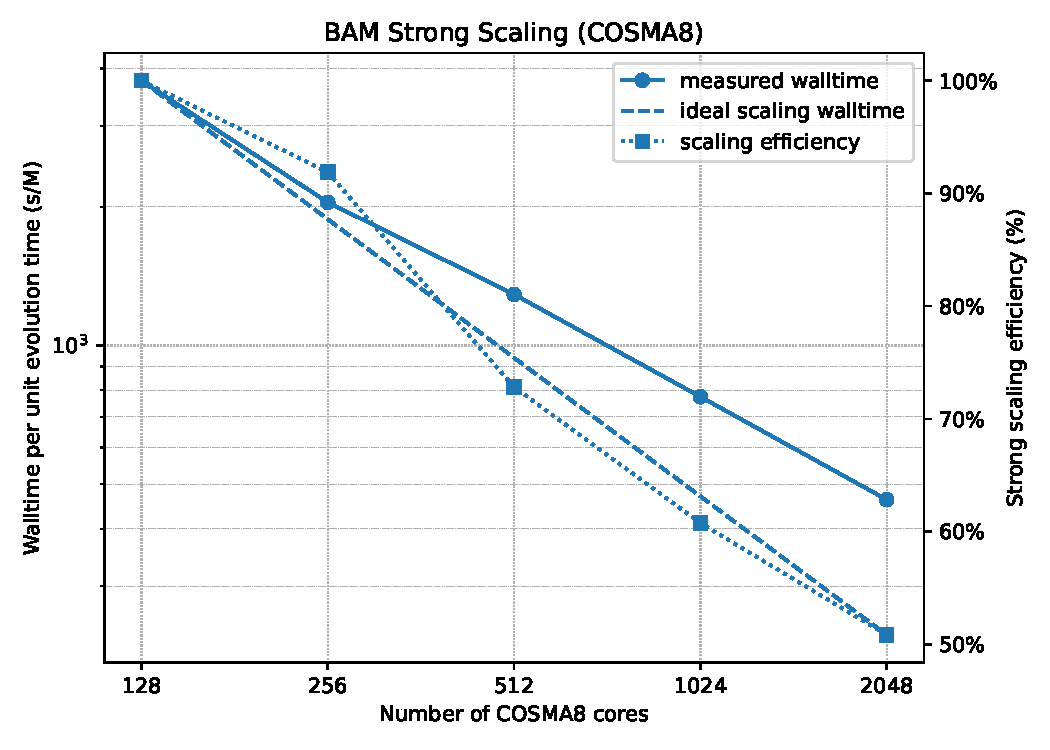
\includegraphics[width=\textwidth]{bam_strong_scaling_cosma8_normalized.pdf}
    \caption{Strong scaling results for \bam on COSMA8. The solid line with
    circle markers is the measured walltime of the evolution (left vertical axis
    scale). The dashed line is the ideal (or perfect) strong scaling walltime
    starting from the measured walltime on 128 cores and assuming perfect
    speedup the number of cores is increased. The dotted line with square
    markers is the scaling efficiency (right vertical axis scale) which is the
    percentage of the ideal speedup achieved by the code as the number of cores
    is increased. In the perfect scaling case, this line would be flat at
    100\%.}
    \label{fig:bam-strong-scaling-cosma8}
\end{figure}

The \bam tests used the following configuration:
\begin{itemize}
    \item 12 levels of mesh refinement (including coarsest level).
    \item 6 levels of fixed boxes and 6 levels of moving boxes.
    \item $320^2 \times 160$ points and $4400^2 \times 2200$ (bitant symmetry)
    length in code units on the coarsest level.
    \item $\sim 1/149$ resolution on the finest level.
    \item 2 timesteps on the coarsest level with subcycling from level 7 onwards
    ($t_{\text{end}} = 0.107421875$).
    \item Due to BAM's data distribution, we were only able to go up to
    16 nodes (2048 cores) on COSMA8 (there was an error with 4096 cores).
\end{itemize}
Full details of the configuration can be found in the
\href{https://github.com/UKNumericalRelativity/uknr-benchmarking/blob/presentation/codes/BAM/COSMA8/inputs/GW150914.par}{BAM 
parameter file}.

The strong scaling result are shown in
Fig.~\ref{fig:bam-strong-scaling-cosma8}. BAM exhibits good strong
scaling up to 2048 cores with a steady decrease in scaling efficiency.

\subsection{Einstein Toolkit scaling}

\begin{figure}[h]
    \centering
    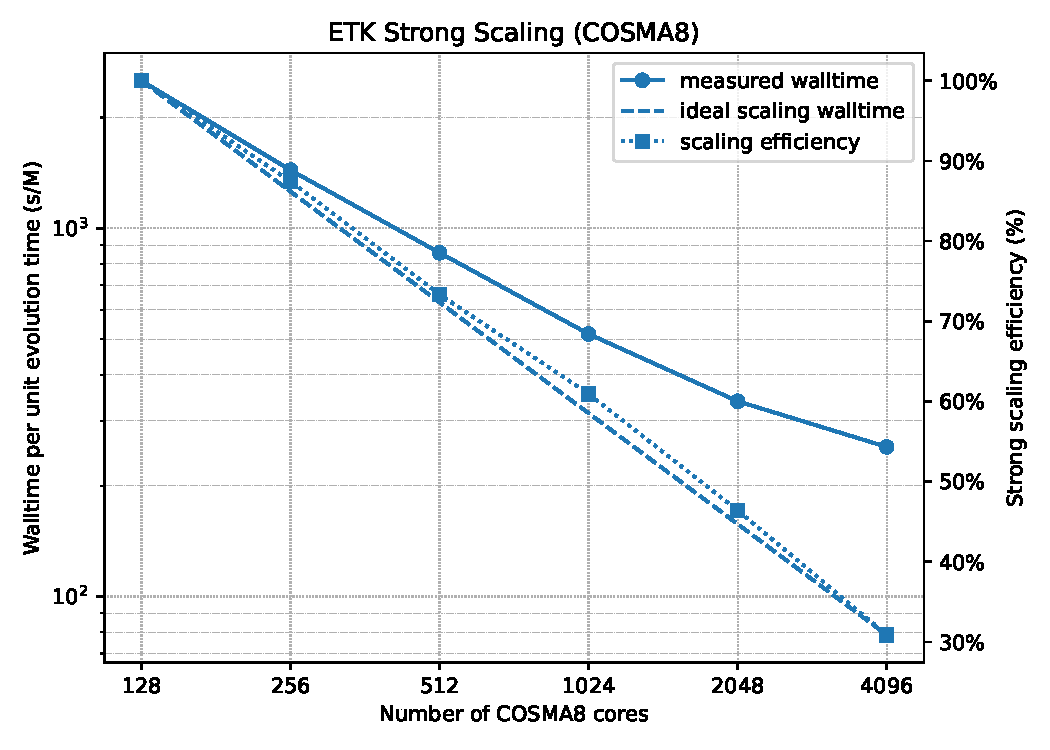
\includegraphics[width=\textwidth]{etk_strong_scaling_cosma8_normalized.pdf}
    \caption{Strong scaling results for the \einsteintoolkit using \carpet on
    COSMA8. The solid line with circle markers is the measured walltime of the
    evolution (left vertical axis scale). The dashed line is the ideal (or
    perfect) strong scaling walltime starting from the measured walltime on 128
    cores and assuming perfect speedup the number of cores is increased. The
    dotted line with square markers is the scaling efficiency (right vertical
    axis scale) which is the percentage of the ideal speedup achieved by the
    code as the number of cores is increased. In the perfect scaling case, this
    line would be flat at 100\%.}
    \label{fig:etk-carpet-strong-scaling-cosma8}
\end{figure}

The \einsteintoolkit tests on COSMA8 used the following configuriation:
\begin{itemize}
    \item 10 levels of mesh refinement (including coarsest level).
    \item $320^2 \times 160$ points and $1024^2 \times 512$ (bitant symmetry)
    length in code units on the coarsest level.
    \item $1/160$ resolution on the finest level.
    \item Subcycling on all but the coarsest two levels.
    \item Terminated after 256 iterations (1 timestep on the coarsest level:
    $t_{\text{end}} = 0.4$).
\end{itemize}
Full details of the configuration can be found in the
\href{https://github.com/UKNumericalRelativity/uknr-benchmarking/blob/presentation/codes/ETK/COSMA8/inputs/GW150914.par}{\etk
COSMA8 parameter file}.

The strong scaling results on COSMA8 are shown in
Fig.~\ref{fig:etk-carpet-strong-scaling-cosma8}. The \einsteintoolkit
exhibits good strong scaling up to the maximum number of cores 
with a steady reduction in scaling efficiency
as the number of cores is increased.

\begin{figure}[h]
    \centering
    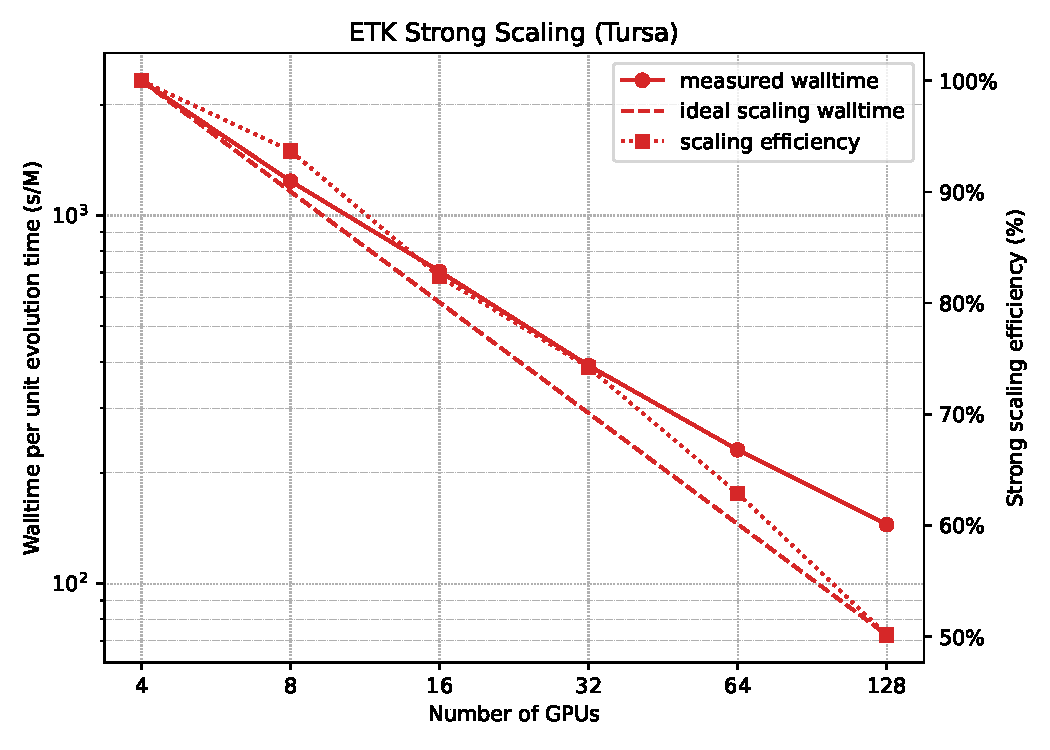
\includegraphics[width=\textwidth]{etk_strong_scaling_tursa_normalized.pdf}
    \caption{Strong scaling results for the \einsteintoolkit using \carpetx on
    Tursa. The solid line with circle markers is the measured walltime of the
    evolution (left vertical axis scale). The dashed line is the ideal (or
    perfect) strong scaling walltime starting from the measured walltime on 4
    GPUs and assuming perfect speedup the number of GPUs is increased. The
    dotted line with square markers is the scaling efficiency (right vertical
    axis scale) which is the percentage of the ideal speedup achieved by the
    code as the number of GPUs is increased. In the perfect scaling case, this
    line would be flat at 100\%.}
    \label{fig:etk-carpetx-strong-scaling-tursa}
\end{figure}

The \einsteintoolkit tests on Tursa used the following configuration:
\begin{itemize}
    \item 10 levels of mesh refinement (including coarsest level).
    \item $288^3$ points and $1024^3$ length in code units on the coarsest
    level (issues with bitant symmetry hence not used).
    \item $1/144$ resolution on the finest level.
    \item Subcycling on all levels.
    \item Terminated after 512 iterations (1 timestep on the coarsest level:
    $t_{\text{end}} \approx 0.889$).
\end{itemize}
Full details of the configuration can be found in the
\href{https://github.com/UKNumericalRelativity/uknr-benchmarking/blob/presentation/codes/ETK/Tursa/inputs/GW150914.par}{\etk
Tursa parameter file}.

The strong scaling results on Tursa are shown in
Fig.~\ref{fig:etk-carpetx-strong-scaling-tursa}. Here, the \einsteintoolkit
exhibits good strong scaling up to 128 GPUs and maintains scaling
efficiency as the number of GPUs increases better than for the CPU version
\carpet on COSMA8. For smaller numbers of
resources, the walltime per unit of evolution time looks similar on both
systems, but this is not a fair comparison since the grid configurations
differ. Even though the resolution for the Tursa \carpetx configuration is
slightly lower, the total number of grid
points is larger than for the COSMA8 \carpet configuration due to the lack of bitant symmetry.
Because of these differences in the grid configuration, we have chosen not to
plot the results on both systems on a single set of axes as we have done for
\grteclyn and \mhduet.

\subsection{GRTeclyn scaling}

\begin{figure}[h]
    \centering
    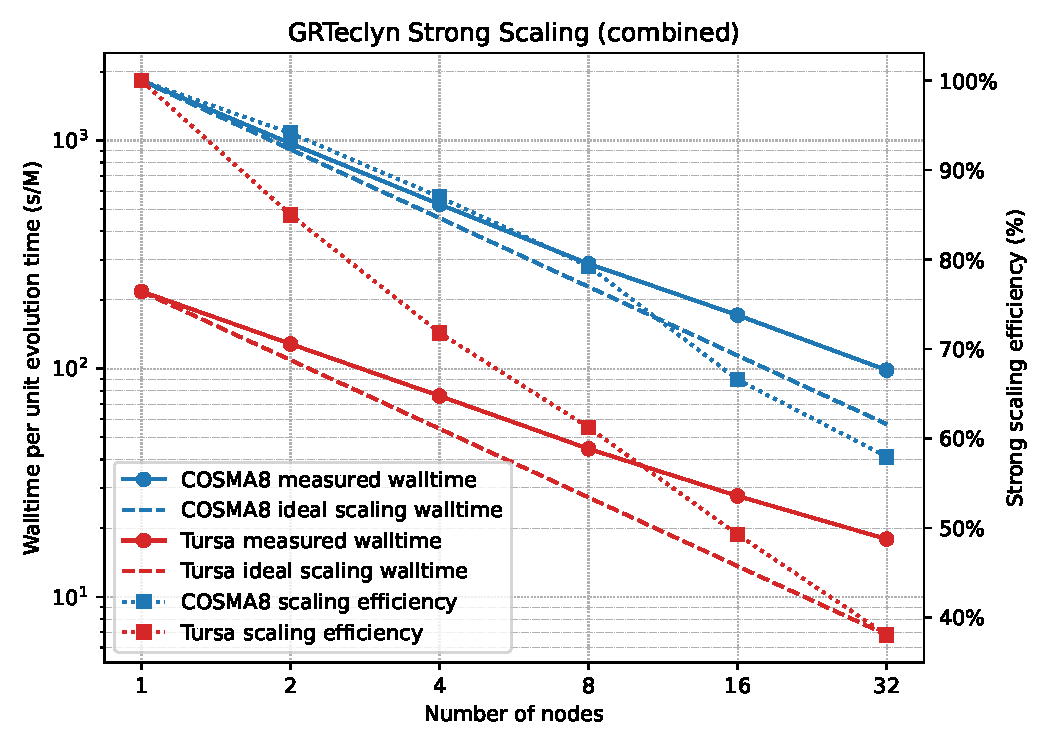
\includegraphics[width=\textwidth]{grteclyn_strong_scaling_combined_normalized_node_aligned.pdf}
    \caption{Strong scaling results for \grteclyn on both COSMA8 and Tursa. The
    COSMA8 results are shown in blue and the Tursa results are shown in red.
    The solid lines with circle markers are the measured walltimes of the
    evolution (left vertical axis scale). The dashed lines are the ideal (or
    perfect) strong scaling walltimes starting from the measured walltime on 1
    node and assuming perfect speedup as the number of nodes is increased. The
    dotted line with square markers is the scaling efficiency (right vertical
    axis scale) which is the percentage of the ideal speedup achieved by the
    code as the number of nodes is increased. In the perfect scaling case, this
    line would be flat at 100\%.}
    \label{fig:grteclyn-strong-scaling-node-aligned}
\end{figure}

\begin{figure}[h]
    \centering
    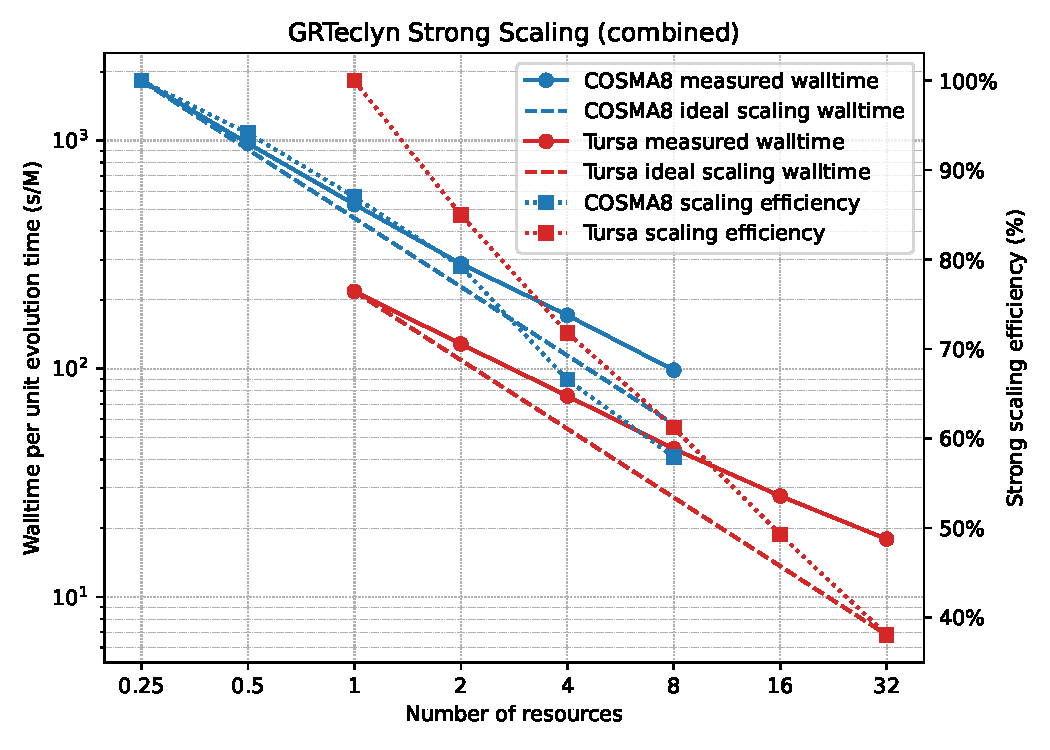
\includegraphics[width=\textwidth]{grteclyn_strong_scaling_combined_normalized_gpu_aligned.pdf}
    \caption{Strong scaling results for \grteclyn on both COSMA8 and Tursa.
    This plot is very similar to
    Fig.~\ref{fig:grteclyn-strong-scaling-node-aligned} but we have aligned the
    results on both systems such that a single node on COSMA8 corresponds to a
    single GPU on Tursa. On the horizontal axis 1 resource is either 4 COSMA8
    nodes or a full Tursa node with 4 GPUs.}
    \label{fig:grteclyn-strong-scaling-gpu-aligned}
\end{figure}

The \grteclyn tests on both systems used the following configuration:
\begin{itemize}
    \item 10 levels of mesh refinement (including coarsest level).
    \item $320^2 \times 160$ cells and $1024^2 \times 512$ (bitant symmetry)
    length in code units on the coarsest level.
    \item $1/160$ resolution on the finest level.
    \item Subcycling on all levels.
    \item 1 timestep on the coarsest level ($t_{\text{end}} = 0.8$).
\end{itemize}
Full details of the configuration can be found in the
\href{https://github.com/UKNumericalRelativity/uknr-benchmarking/blob/presentation/codes/GRTeclyn/Tursa/inputs/params_GW150914.txt}{\grteclyn
parameter file}.

The strong scaling results on both systems are shown in both
Fig.~\ref{fig:grteclyn-strong-scaling-node-aligned} and
Fig.~\ref{fig:grteclyn-strong-scaling-gpu-aligned}. The former shows the results
aligned such that 1 COSMA8 node is equivalent to 1 Tursa node (4 GPUs) which is
the more conventional approach when comparing between GPUs and CPUs. The latter
shows the results aligned such that 1 COSMA8 node is equivalent to a single
Tursa GPU which is often argued to be a fairer comparison when you take into account
the power usage and purchase cost of the hardware.

On COSMA8, \grteclyn exhibits good strong scaling up to 32
nodes (4096 cores) with a decreasing scaling efficiency dropping to $~58\%$ for the largest job size.
%with the highest scaling efficiency at the largest job size of the codes we tested ($~58\%$). 
On Tursa GPUs, scaling efficiency drops more
quickly than on COSMA8 CPUs but the walltime per unit of
evolution time is lower which suggests that there may be
insufficient work per GPU for the larger Tursa job sizes.

\subsection{MHDuet scaling}

\begin{figure}[h]
    \centering
    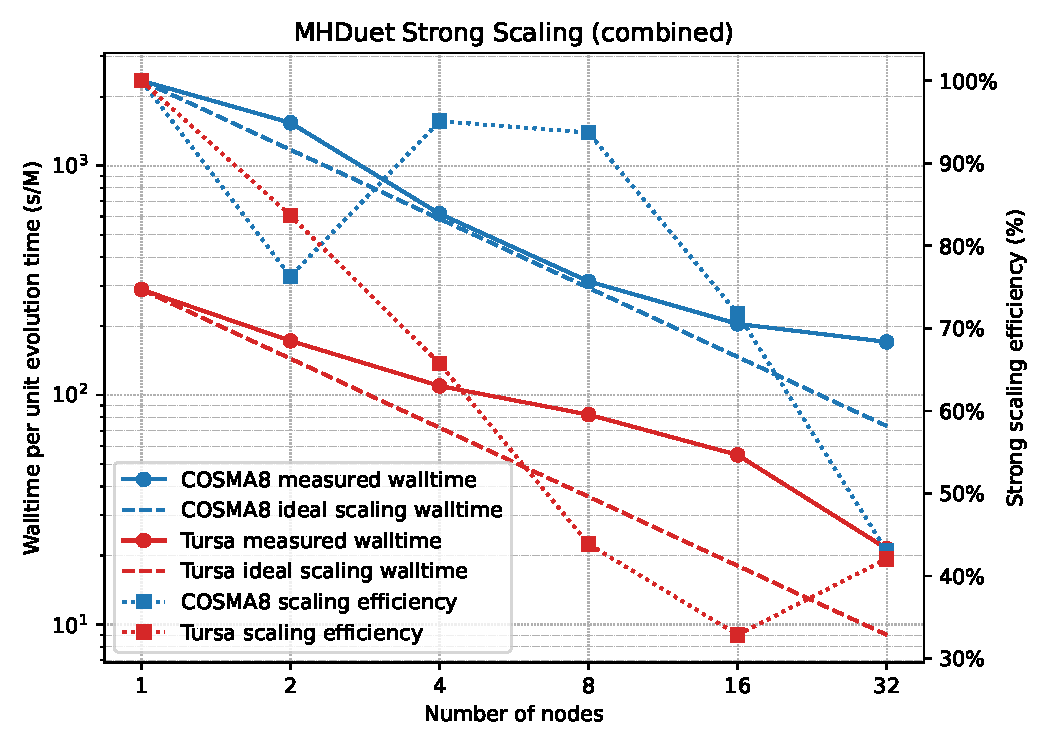
\includegraphics[width=\textwidth]{mhduet_strong_scaling_combined_normalized_node_aligned.pdf}
    \caption{Strong scaling results for \mhduet on both COSMA8 and Tursa. The
    COSMA8 results are shown in blue and the Tursa results are shown in red.
    The solid lines with circle markers are the measured walltimes of the
    evolution (left vertical axis scale). The dashed lines are the ideal (or
    perfect) strong scaling walltimes starting from the measured walltime on 1
    node and assuming perfect speedup as the number of nodes is increased. The
    dotted line with square markers is the scaling efficiency (right vertical
    axis scale) which is the percentage of the ideal speedup achieved by the
    code as the number of nodes is increased. In the perfect scaling case, this
    line would be flat at 100\%.}
    \label{fig:mhduet-strong-scaling-node-aligned}
\end{figure}

\begin{figure}[h]
    \centering
    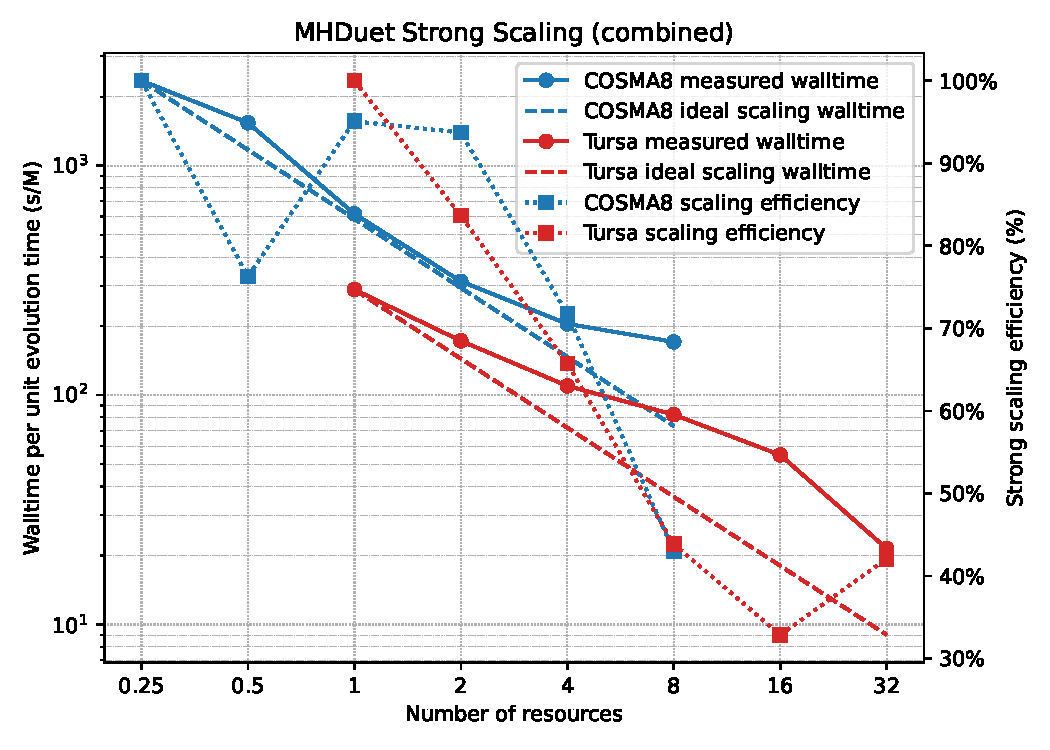
\includegraphics[width=\textwidth]{mhduet_strong_scaling_combined_normalized_gpu_aligned.pdf}
    \caption{Strong scaling results for \mhduet on both COSMA8 and Tursa.
    This plot is very similar to
    Fig.~\ref{fig:mhduet-strong-scaling-node-aligned} but we have aligned the
    results on both systems such that a single node on COSMA8 corresponds to a
    single GPU on Tursa. On the horizontal axis 1 resource is either 4 COSMA8
    nodes or a full Tursa node with 4 GPUs.}
    \label{fig:mhduet-strong-scaling-gpu-aligned}
\end{figure}

The \mhduet tests on both systems used the following configuration:
\begin{itemize}
    \item 10 levels of mesh refinement (including coarsest level).
    \item $256^3$ cells and $1024^3$ length in code units on the coarsest level.
    \item Fixed mesh refinement for the coarsest 6 levels with boxes of lengths:
    1024, 512, 256, 128, 64, 32
    \item $1/128$ resolution on the finest level.
    \item Subcycling on all levels.
    \item 1 timestep on the coarsest level ($t_{\text{end}} = 1.6$).
\end{itemize}
Full details of the configuration can be found in the
\href{https://github.com/UKNumericalRelativity/uknr-benchmarking/blob/presentation/codes/MHDuet/Tursa/inputs/GW150914.input}{\mhduet
parameter file}.

The strong scaling results on both systems are shown in both
Fig.~\ref{fig:mhduet-strong-scaling-node-aligned} and
Fig.~\ref{fig:mhduet-strong-scaling-gpu-aligned}. The former shows the results
aligned such that 1 COSMA8 node is equivalent to 1 Tursa node (4 GPUs) which is
the more conventional approach when comparing between GPUs and CPUs. The latter
shows the results aligned such that 1 COSMA8 node is equivalent to a single
Tursa GPU which is often argued to be a fairer comparison when you take into account
the power usage and purchase cost of the hardware.

\mhduet exhibits very good scaling on COSMA8 up to 16 nodes (2048
cores) with a slightly larger drop when moving to 4096 cores. On Tursa, the
scaling is also good, dropping beyond 4 nodes (16 GPUs) but then improving slightly
at 32 nodes (128 GPUs). The scaling efficiency is unusual since we normally expect this to monotonically
decrease as the number of resources is increased. Non-monotonic scaling
behaviour can sometimes be explained by a threshold effect e.g. the work per
core exceeds one of the cache sizes and so the performance improves by more than
the proportionate increase in resources when moving to a a larger number of
cores. The developers may wish to investigate this further. 
As with GRTeclyn, the scaling efficiency is low at the larger job sizes
which suggests that there may be
insufficient work per GPU in these cases.

\subsection{Profiling}

\begin{figure}[h]
    \centering
    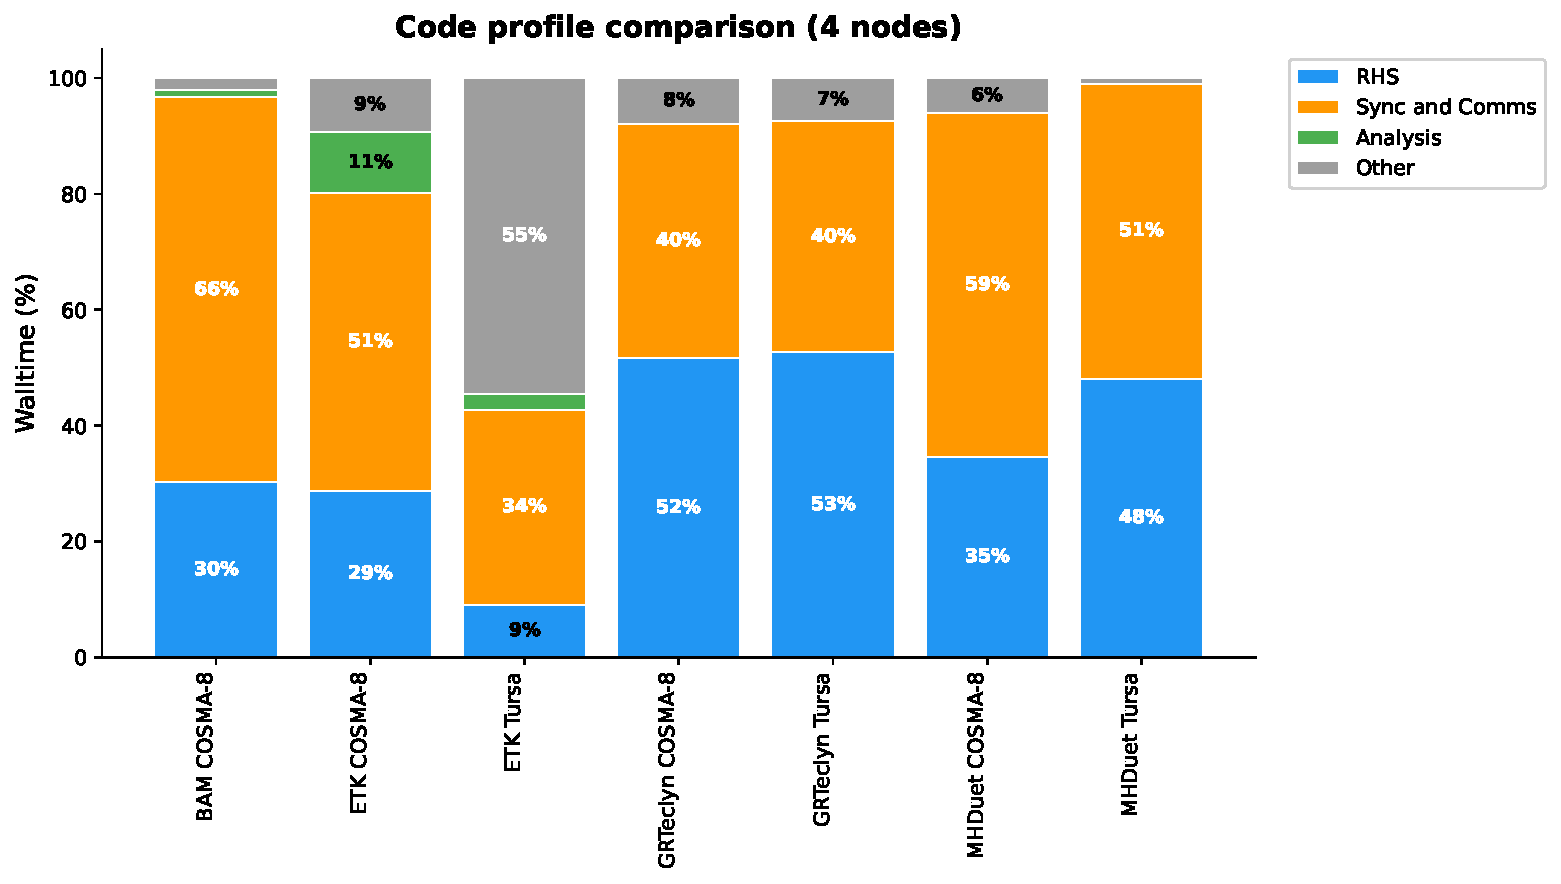
\includegraphics[width=\textwidth]{profile_comparison_4nodes.pdf}
    \caption{Profiling results for all codes on 4 nodes on either COSMA8 or
    Tursa as labelled. For each code, we used its internal profiling/timer infrastructure
    to obtain the walltime spent in relevant parts of the code. ``RHS'' includes
    evaluation of the RHS and enforcement of any algebraic constraints but does
    not include any time spent in time integration. ``Sync and Comms'' includes
    any time spent in interpolation/restriction/prolongation between levels as
    well as communication of ghost zones between MPI processes. ``Analysis''
    includes anything that is not strictly necessary for evolution. This
    includes but is not limited to calculation of constraints and $\Psi_4$,
    apparent horizon finding, calculation of ADM variables, and puncture
    tracking. Note that the latter may be deemed necessary in order to track BHs
    for moving boxes/refinement but we have decided to include it under
    ``Analysis'' for the sake of comparison. For any walltime not accounted for
    in these categories, we have included it under ``Other''.}
    \label{fig:profiling-comparison}
\end{figure}

In addition to performing strong scaling tests, we also enabled internal
profilers/timers in each of the codes so that we could obtain a breakdown of the
walltime spent in different parts of the code. A stacked bar chart of these
profiles for the simulations on 4 nodes is shown in
Fig.~\ref{fig:profiling-comparison}. Note that due to the differences in the
structures of the code, the categories used are relatively broad:
\begin{itemize}
    \item ``RHS'': evaluation of the right-hand side and enforcement of any
    algebraic constraints but does not include any time spent in time
    integration
    \item ``Sync and Comms'': any time spent in
    interpolation/restriction/prolongation between levels as well as
    communication of ghost zones between MPI processes.
    \item ``Analysis'': any time spent in routines that are not strictly
    necessary for evolution. This includes but is not limited to calculation of
    constraints and $\Psi_4$, apparent horizon finding, calculation of ADM
    variables, and puncture tracking (even though this may be deemed necessary
    in order to track BHs for moving boxes/refinement, we have decided to
    include it under ``Analysis'' for the sake of comparison).
    \item ``Other'': Any walltime not accounted for in the above categories.
\end{itemize}
If the analysis were to be restricted to an individual code, it would be
possible to obtain a profile with more detailed categories. Note that we have
also scaled all bars to the same height rather than by the total walltime for
each code since the grid configurations differ.

From this chart alone, it is difficult to draw concrete conclusions about the
opportunity for potential optimizations. However, by combining the information
from this chart with the strong scaling results and inspection of the code's
structure, we can make some observations:
\begin{itemize}
    \item A relatively large fraction of the walltime is spent in ``Sync and
    Comms'' for \bam. Looking at the communication patterns in the code, it
    seems that individual variables are typically communicated separately and
    one potential optimization would be to combine these into a single call and
    consider exploiting non-blocking/asynchronous communication.
    \item
    \begin{sloppypar} % to fix the ODESolvers_Solve_Subcycling line breaking
    Most of the time of the \etk \carpetx code is spent in the ``other'' category. 
    From the timer output, much of this is in the
    \texttt{ODESolvers\_Solve\_Subcycling} routine. Only a small fraction of
    this routine is spent in the actual RHS calculation. Our
    tests were performed using a development version of \carpetx so
    these results probably do not reflect what would be observed with the main
    repository once subcycling support is finalised\footnote{At the time of
    writing, there is an
    \href{https://github.com/EinsteinToolkit/CarpetX/pull/371}{open pull
    request} to add this capability.}, or in a non-subcycling version of the code. 
    We expect the profile to be more comparable to the
    other codes once optimisation of this routine is complete.
    \end{sloppypar}
    \item From the chart we can see that \grteclyn spends the greatest fraction
    of its time in the RHS evaluation. Efforts to optimize this part of the code
    are currently ongoing and we expect this fraction to decrease soon.
    \item Analysis of the timer output from \mhduet shows that there is a discrepancy
    between the minimum and maximum walltimes of e.g. the RHS evaluation across
    MPI processes, which suggests the existence of load
    imbalance. This may partially explain the non-monotonic scaling behaviour
    observed in Fig.~\ref{fig:mhduet-strong-scaling-node-aligned}.
\end{itemize}


%=============================================================================
\section{Conclusion}
\label{sec:conclusion}

In this report, we have presented an assessment of the 3+1 numerical
relativity codes that are developed and used by members of the UKNR
community, carried out in anticipation of a potential UKNR Collaborative
Computational Project (CCP). We assessed five codes: \bam, the
\einsteintoolkit, \exagrype, \grteclyn and \mhduet. In Sec.~\ref{sec:codes},
we described their current capabilities, including their numerical and
mathematical methods. Despite being built on very different infrastructures,
they share many common ingredients such as finite differences, hierarchies of
Cartesian mesh refinement levels, Method of Lines time integration and a
BSSN, CCZ4 or Z4c formulation with moving puncture gauge conditions. After
briefly describing the DiRAC HPC systems (COSMA8 and Tursa) used for testing
in Sec.~\ref{sec:hpc}, we documented our qualitative experiences of
obtaining, building and using each code in Sec.~\ref{sec:usability}, and
presented strong scaling tests and profiling of each code in
Sec.~\ref{sec:performance}. Here, we summarise our main findings for each
code.

\begin{description}
    \item[\bam.] Of the codes we assessed, \bam was the most straightforward to
    build and run, thanks to its very small number of dependencies, its
    conventional Makefile build system (which only required straightforward
    modifications to the template configuration file) and its conventional
    launch workflow. It is also the code with the longest history and,
    reflecting this, it is written in an older style of C: building it with a
    modern compiler required a few adjustments that are well understood for
    long-lived C codes (e.g. adding the \texttt{-fcommon} flag and some function
    forward declarations). The documentation included with the code provides
    some basic information but has not been updated in some time, so new users
    will likely benefit from guidance from experienced users when exploring the
    available parameters. We also did not find a supported output format that
    permits visualization across the full mesh refinement hierarchy. \bam would 
    benefit from dedicated RSE support to modernize the codebase
    and improve its documentation. On the performance side, \bam exhibited
    relatively good strong scaling on COSMA8 up to 2048 cores (16 nodes), albeit
    with a steady decrease in efficiency; an issue related to its data
    distribution prevented us from running on more cores. Profiling revealed
    that the largest fraction ($\sim 2/3$) of its walltime is spent in
    synchronization and communication. Since individual grid variables appear to
    be communicated separately, combining these into fewer (and potentially
    non-blocking/asynchronous) communications is a promising optimization
    opportunity.

    \item[\einsteintoolkit.] The \einsteintoolkit offers the widest range of
    features and the greatest flexibility of the codes we tested. 
    This richness naturally comes with some additional complexity -- for example, 
    obtaining the code requires assembling a thornlist, and
    configuring \textsc{SimFactory2}, which can be a challenge for a system that is not in its machine
    database. Builds can be
    slow when many thorns are enabled, and documentation coverage varies
    between thorns. We found the ability to print all parameters with
    descriptions, default values and valid ranges particularly helpful and
    believe other codes would benefit from a similar capability. The
    next-generation \carpetx driver used for our GPU tests is still under
    active development, so we used a development version with subcycling
    support and, as is often the case when testing actively developed code,
    needed to invest some effort in resolving runtime issues. On
    COSMA8 with \carpet, the \etk exhibited good strong scaling, with
    an efficiency of $\sim 30\%$ at 4096 cores. On Tursa with \carpetx,
    it exhibited good strong scaling up to 128 GPUs, achieving the best
    GPU-side scaling efficiency ($\sim 60\%$ at 128 GPUs) of the codes we
    tested. The \carpetx profile is dominated by time spent in the subcycling
    driver routine outside of the RHS evaluation, but we emphasize that this
    reflects a development version of the code rather than the main
    repository, so we expect the profile to become more comparable to the
    other codes once subcycling support is merged and optimized.

    \item[\exagrype.]
    \begin{sloppypar} % to fix overfull hbox from ExaHyPE 2/Peano line breaking
    \exagrype takes a distinctive approach: the user
    interacts with a Python domain-specific language built on \exahype
    2/\peano, from which the simulation C++ code is generated and built. 
    Its documentation is
    relatively detailed and helpful, and the Python DSL is designed to make
    it straightforward for users to implement new physics. In its current
    state, however, \exagrype exposes relatively few parameters to the user:
    choices such as the grid configuration, initial data parameters, gauge
    parameters and CCZ4 damping parameters are baked into the source, which
    makes them harder for new users to discover and adjust, and the absence
    of runtime parameters adds some friction when trying different
    configurations. Support for offloading to Nvidia GPUs is under active
    development; at the time of testing we were not yet able to run \exagrype
    with either the SYCL or OpenMP backends on Tursa's Nvidia GPUs, so we did
    not report any scaling results for it.
    \end{sloppypar}

    \item[\grteclyn.] \grteclyn combines a lightweight codebase with
    a conventional and straightforward user experience. It is open source,
    has very few dependencies, builds reasonably quickly using \amrex's
    Makefile build system with minimal configuration, launches in the
    conventional way, has reasonably detailed documentation, and
    offers robust GPU support across Nvidia, AMD and Intel hardware. As a
    relatively new code, several key capabilities (e.g. apparent horizon
    finding) are still under development. \grteclyn exhibited good strong scaling on COSMA8,
    retaining scaling efficiency of $\sim 58\%$ at the largest job size of 32 nodes (4096 cores). On Tursa, its
    scaling efficiency dropped more quickly, but its walltime
    per unit evolution time was lower, suggesting there is
    insufficient work per GPU at the larger job sizes. Profiling shows that
    \grteclyn spends the largest fraction ($\sim 50\%$) of its walltime in the
    RHS evaluation; 
    efforts to optimize this part of the code are ongoing.

    \item[\mhduet.] \mhduet is generated using the \simflowny infrastructure
    and is primarily targeted at MHD and boson star spacetimes; reflecting
    this focus, some capabilities typically used by BBH-oriented codes (e.g.
    puncture tracking) are outside the scope of the generated setup we
    tested. Running a generated \mhduet code is conventional and straightforward, with the build process requiring some system specific customisation of the Makefile. Autogenerated
    code allows users to rapidly implement new physics, but can lead to longer compile times and 
    reduces code readability. The automatically generated documentation focuses on the equations
    being solved and the discretization scheme. \mhduet exhibited very good
    strong scaling on COSMA8 up to 16 nodes (2048 cores), with a
    non-monotonic scaling efficiency, followed by a larger drop when moving
    to 32 nodes (4096 cores). On Tursa, the scaling dropped
    beyond 4 nodes (16 GPUs) before recovering slightly at 32 nodes (128
    GPUs). Analysis of its internal timers indicates some load imbalance, 
    which may partially explain this
    non-monotonic scaling-efficiency behaviour.
\end{description}

Some common themes emerge across all of the codes. The quality and quantity
of documentation varies considerably, and the ease with which a new user can
get started depends heavily on it; essentially all of the codes would benefit
from further RSE investment, with the longest-established codes having the
most to gain. The codes built on \amrex (\grteclyn, \mhduet and the \etk with
\carpetx) provide the most straightforward and portable GPU support. On GPUs,
the walltime per unit evolution time was generally lower than on CPUs at
comparable resource counts, but scaling efficiencies dropped faster, indicating
that larger problems are needed to saturate GPU-based systems.  Finally, we
reiterate that many of these codes are under active development, so this
assessment is only a snapshot in time.

Given more time and resources, there are several directions we would like to
pursue:
\begin{itemize}
    \item Weak scaling analysis: our performance tests were restricted to strong
    scaling at a fixed problem size. Weak scaling tests, where the problem size
    is increased in proportion to the computational resources, would reveal how
    well the codes exploit much larger partitions. In practice, the simulation
    configurations used here for our strong scaling tests are already at the
    larger end of what is typically used in production simulations for similar mass ratio binaries.
    \item Accuracy comparison between the codes of a full BBH simulation: we
    only evolved each configuration for a few timesteps. Evolving a complete
    inspiral, merger and ringdown of a fixed binary configuration (e.g. the
    GW150914-based setup used here) with each code and comparing the results
    (e.g. extracted gravitational waveforms and horizon diagnostics) would
    enable a direct accuracy comparison between the codes, complementing
    existing two-code comparisons in the literature.
    \item Resources required to achieve the same accuracy: combining such an
    accuracy study with performance measurements would allow us to determine
    the computational resources (e.g. core-hours or GPU-hours, and by
    extension financial and energy cost) that each code requires to reach a
    common accuracy target. We believe this is ultimately the most meaningful
    metric for comparing performance between codes, since comparing
    walltimes at similar grid resolutions is not like-for-like if the codes
    achieve different accuracies.
    \item Extending the assessment beyond vacuum black hole spacetimes to
    include matter, and repeating the assessment as the newer codes continue
    to mature (e.g. once \carpetx gains merged subcycling support, \exagrype
    gains Nvidia GPU support, and \grteclyn's remaining capabilities such as
    apparent horizon finding are completed).
\end{itemize}

\section*{Acknowledgements}

We thank the STFC DiRAC HPC Facility for providing compute resources on Tursa
and COSMA8. For \bam, we thank Rhiannon Silva for providing
a suitable parameter file and helpful discussions. For the \einsteintoolkit, we
thank Patricia Schmidt and Geraint Pratten for discussions on ETK Carpet thorns
they use for their simulations, and the wider Einstein Toolkit community,
particularly Roland Haas and Liwei Ji, for their support in resolving issues
with CarpetX. For \exagrype, we thank Han Zhang, Tim Stokes and Tobias
Weinzierl for support in getting started with ExaGRyPE. For \mhduet, we thank
Carlos Palenzuela for generating a suitable code for binary black-hole
evolution and Miguel Bezares for implementation support. We also thank the wider UKNR community for helpful discussions and feedback. This work is supported by a UKRI Collaborative Computational Project grant UKRI496, and a SHAREing grant RF090191.  


\printbibliography

\end{document}
